%%%%%%%%%%%%%%%%%%%%%%%%%%%%%%%%%%%%%%%%%%%%%%%%%%%%%%%%%%%%%%%%%%%%%
%  Executar:   pdflatex
%              bibtex
%              pdflatex
%              pdflatex
%%%%%%%%%%%%%%%%%%%%%%%%%%%%%%%%%%%%%%%%%%%%%%%%%%%%%%%%%%%%%%%%%%%%%
%  DMTeX
%
%  Arquivo LaTeX para formatação de TCC, Mestrado e Doutorado
%  TCC, PPGM, PPGECE, ProfMat segundo as normas ABNT
%
%  Departamento de Matemática - UFSCar
%
%  Autor: Wladimir Seixas (seixas@ufscar.br)
%  Última atualização: 25/11/2021
%
%  Pacotes LaTeX que já estão carregados:
%
%     fontenc		helvet			inputenc		babel
%     microtype		geometry		setspace		graphicx
%     float			indentfirst		fancyhdr		etoolbox
%     caption		footmisc		enumitem		tocloft
%     amsmath		amsfonts		amssymb			amsthm
%     varioref		hyperref		color			backref
%     abntex2cite	appendix		mdframed        pdfpages
%     imakeidx
%
% Já estão pré-definidos os seguintes ambientes:
%
%	 \begin{teorema} .... \end{teorema}
%	 \begin{lema} .... \end{lema}
%	 \begin{proposicao} .... \end{proposicao}
%	 \begin{corolario} .... \end{corolario}
%	 \begin{definicao} .... \end{definicao}
%	 \begin{conjectura} .... \end{conjectura}
%	 \begin{exemplo} .... \end{exemplo}
%
%    Arquivos: dmtex.cls (template LaTeX)
%              monografia.tex 
%              referencias.bib (database BibTeX)
%              arquivosdmtex (diretório contendo logos)
%
%%%%%%%%%%%%%%%%%%%%%%%%%%%%%%%%%%%%%%%%%%%%%%%%%%%%%%%%%%%%%%%%%%%%%
%  PREENCHER OS APENAS OS CAMPOS DE INFORMAÇÕES
%  NÃO ALTERAR A ORDEM DOS COMANDOS. 
%  A CONFECÇÃO DO TRABALHO SEGUE A ORDEM DEFINIDA NA ABNT   
%%%%%%%%%%%%%%%%%%%%%%%%%%%%%%%%%%%%%%%%%%%%%%%%%%%%%%%%%%%%%%%%%%%%%

% CURSO          OPÇÃO
% TTC            tcc
% PROFMAT        profmat
% PPGECE         ppgece
% PGM-MESTRADO   mestre
% PGM-DOUTORADO  doutor

% Escolher uma das opções (% caso não se aplique).
%\documentclass[tcc,licenciatura]{dmtex}
\documentclass[tcc,bacharelado]{dmtex}
%\documentclass[ppgece]{dmtex}
%\documentclass[profmat,nofont]{dmtex}
%\documentclass[mestre,nofont]{dmtex}
%\documentclass[doutor,nofont]{dmtex}

% Coloque aqui outros pacotes LaTeX que você faça uso 
% (ver tabela acima)
\usepackage{enumitem}
% \usepackage[•]{•}


\begin{document}

%%%%%%%%%%%%%%%%%%%%%%%%%%%%%%%%%%%%%%%%%%%%%%%%%%%%%%%%%%%%%%%%%%%%%
% DADOS: Preencher os campos comentando caso não se aplique.
%%%%%%%%%%%%%%%%%%%%%%%%%%%%%%%%%%%%%%%%%%%%%%%%%%%%%%%%%%%%%%%%%%%%%
 
% Título do trabalho
\titulo{Título do trabalho $\mathbb{R}^n$}

% Autoria - seu nome
\autoria{Nome do autor(a)}

% Ano da defesa depósito
\ano{2021}

% Orientação - preencha o campo correspondente
\orientador{Nome do Orientador}
%\orientadora{Nome da orientadora}
%\coorientador{Nome da coorientador}
%\coorientadora{Nome da coorientadora}

% A capa é um elemento OBRIGATÓRIO 
\capa

%%%%%%%%%%%%%%%%%%%%%%%%%%%%%%%%%%%%%%%%%%%%%%%%%%%%%%%%%%%%%%%%%%%%%
% Elementos pré-textuais
% Parte que antecede o texto com informações que auxiliam na 
% identificação e utilização do trabalho.
%%%%%%%%%%%%%%%%%%%%%%%%%%%%%%%%%%%%%%%%%%%%%%%%%%%%%%%%%%%%%%%%%%%%%

% Folha de Rosto
% A folha de rosto é um elemento OBRIGATÓRIO que apresenta os 
% elementos essenciais para identificação do trabalho.
%\folhaderosto

% A ficha catalográfica, elemento OBRIGATÓRIO em trabalhos 
% acadêmicos, segundo a Norma ABNT - NBR 14724/2011 
% (Informação e documentação – Trabalhos acadêmicos – 
% apresentação), deve ser inserida no verso da folha de 
% rosto (na parte inferior). Para obter a ficha é necessário 
% que o autor preencha os campos com os dados da sua monografia, 
% o programa fará a formatação correta dos dados e irá gerar 
% a ficha catalográfica em um arquivo .PDF, fazendo o download 
% automático.
% Acesso: https://www.sibi.ufscar.br/servicos/gerador-de-ficha-catalografica
\thispagestyle{empty}
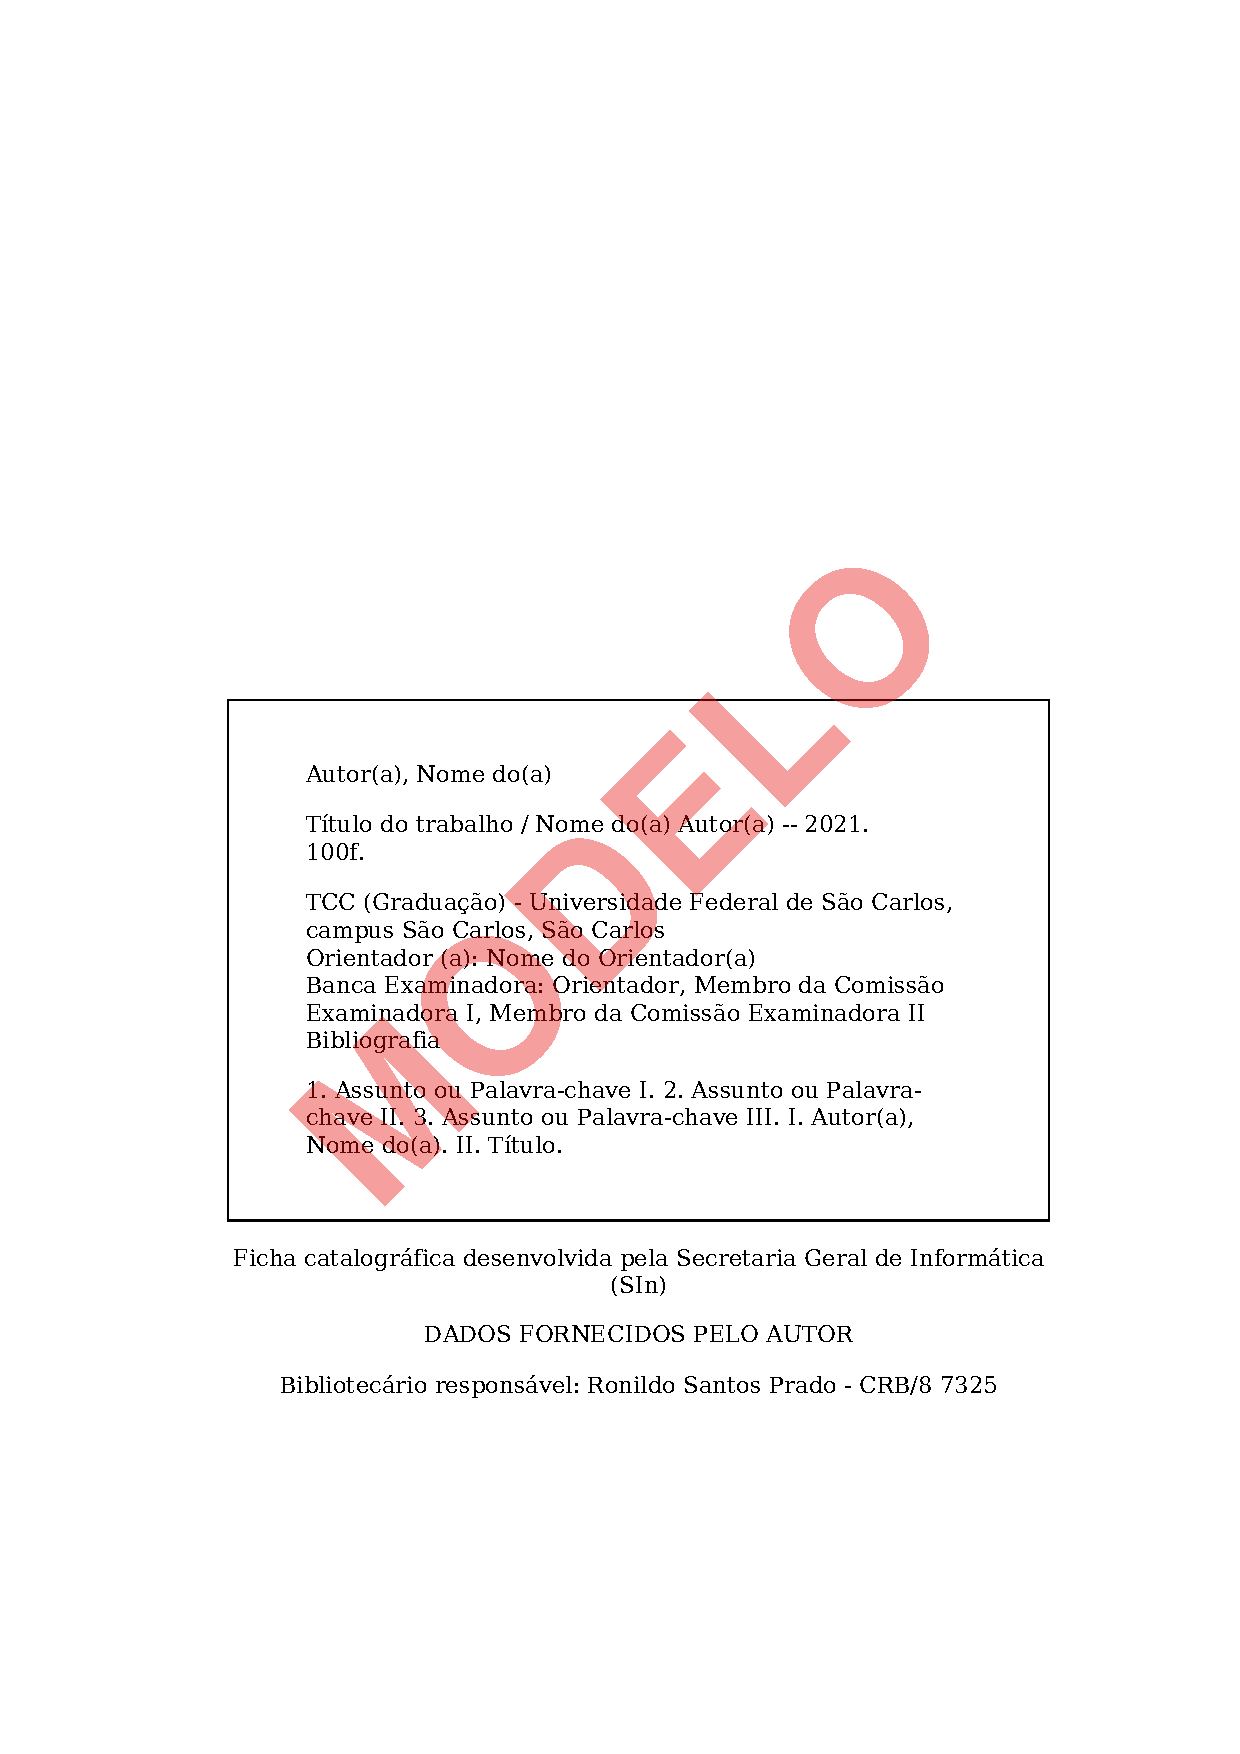
\includepdf[width=1.1\textwidth]{ficha-catalografica.pdf}

% A folha de aprovação é elaborada e fornecida pela 
% Coordenação de Curso (TCC) ou pelo 
% Programa de Pós-Graduação (PPGECE, Profmat ou PPGM)
\thispagestyle{empty}
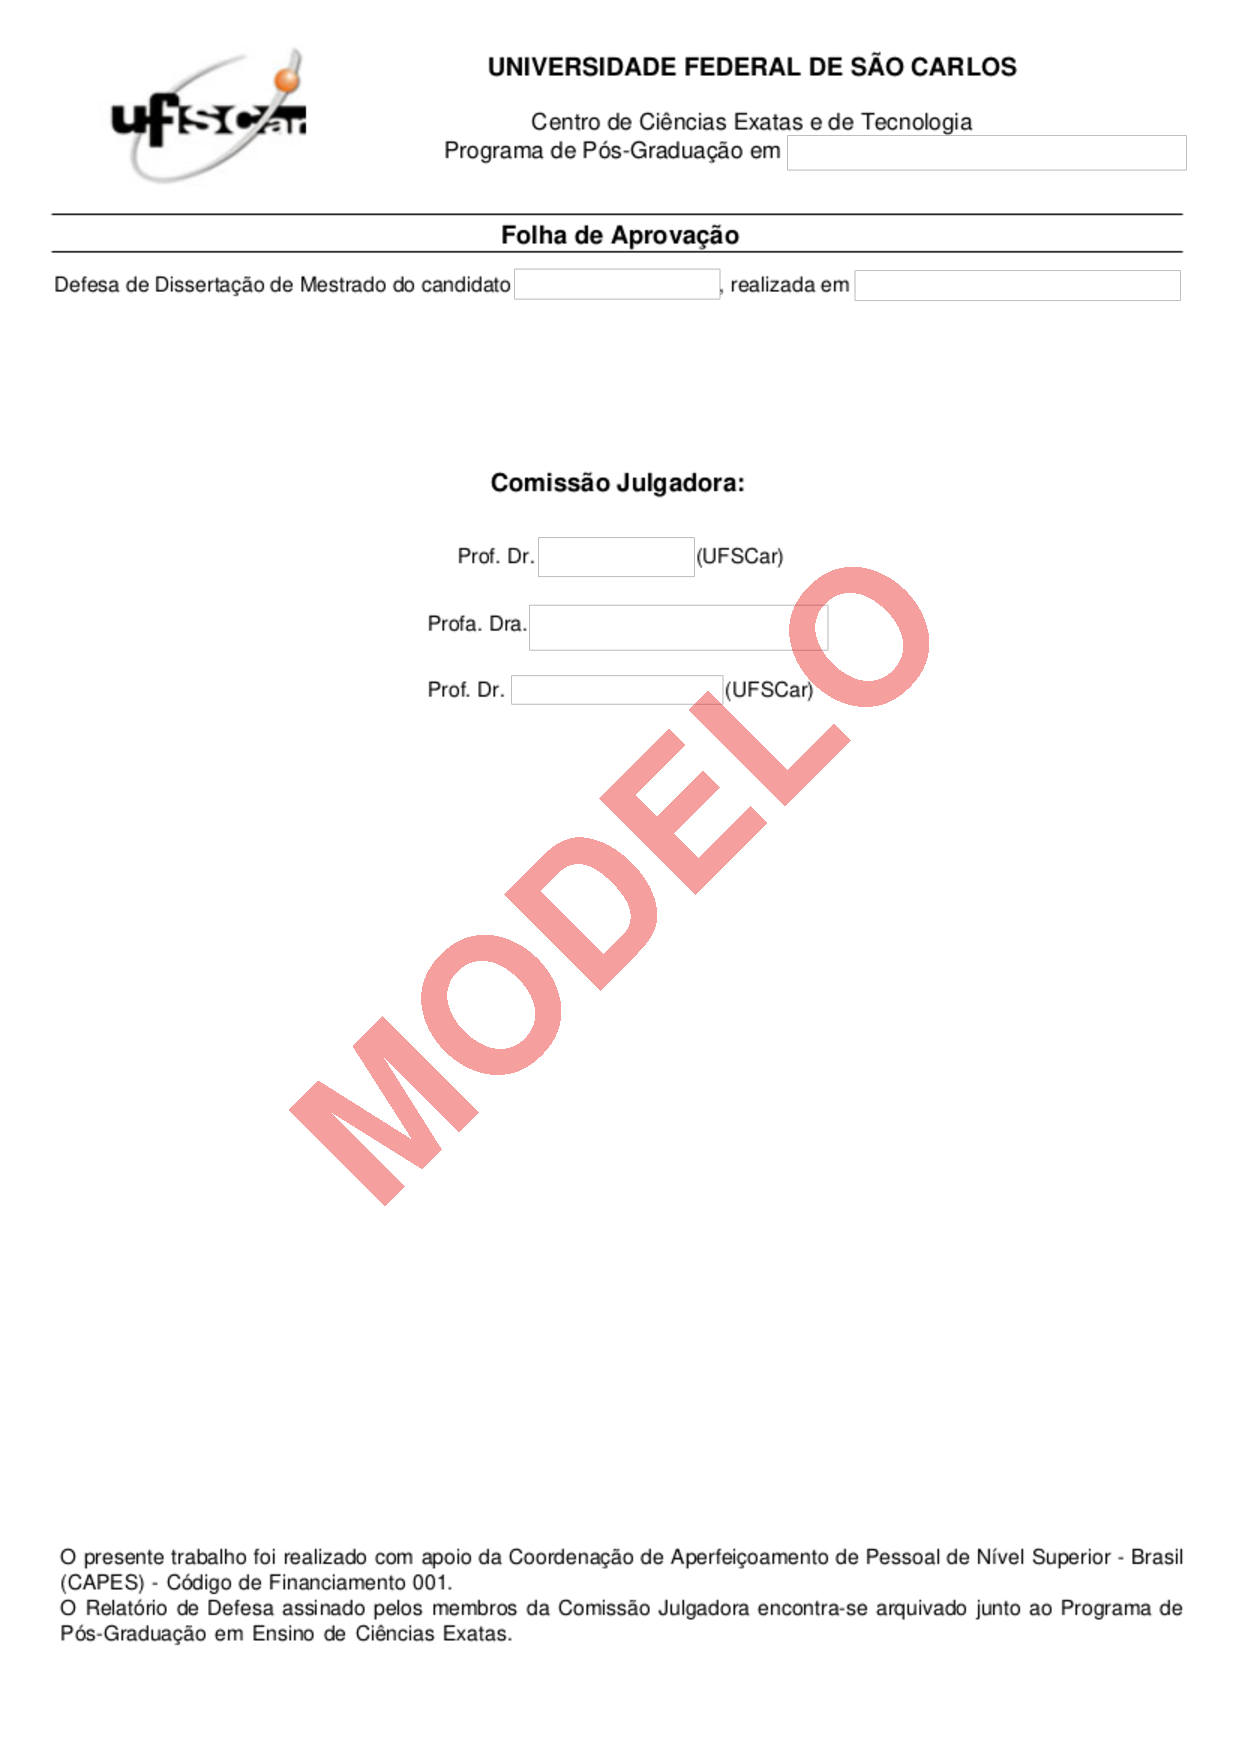
\includepdf[width=1.1\textwidth]{folhadeaprovacao.pdf}

% Dedicatória
% Comente o ambiente a seguir caso não fizer uso.
\begin{dedicatoria}

A dedicatória é um elemento OPCIONAL em que \\ o autor presta homenagem ou dedica seu trabalho.

\end{dedicatoria}

% Agradecimento
% Comente o ambiente a seguir caso não fizer uso.
\begin{agradecimentos}

É um elemento OPCIONAL em que o autor faz agradecimentos aos que contribuíram de
maneira relevante à elaboração do trabalho.

\end{agradecimentos}

% Epígrafe
% É um elemento OPCIONAL em que o autor pode apresentar uma citação. 
% Deve-se fazer a indicação de autoria (citação) e a referência deve 
% constar na lista de Referências no final do trabalho.
% Comente o ambiente a seguir caso não fizer uso.
\begin{epigrafe}
Demonstração: Evidente \\
\textbf{Elon Lages Lima} \cite[p. 154]{elon}.
\end{epigrafe}

% Até 5 palavras-chaves - preencha os campos apropriados
% {1o campo-> em português}{2o campo-> em inglês}
\palavrachaveI{Chave 1}{Key 1}
\palavrachaveII{Chave 2}{Key 2}
\palavrachaveIII{Chave 3}{Key 3}
%\palavrachaveIV{Chave 4}{Key 4}
%\palavrachaveV{Chave 5}{Key 5}

% Resumo na língua vernácula (Português)
\begin{resumo}
Elemento OBRIGATÓRIO, deve apresentar os pontos relevantes do texto, de forma
concisa e que permita uma visão rápida e clara do conteúdo e das conclusões do
trabalho. Indica-se que o resumo tenha no máximo 500 palavras e deve ser
elaborado de acordo com ABNT NBR 6028/2003. Abaixo do resumo devem ser 
colocadas as palavras-chave. A indicação Palavra-chave deve ser em negrito 
seguida de dois pontos e espaço. Cada palavra deve ser separada uma da outra 
por ponto final.
\end{resumo}

% Resumo em língua estrangeira (Inglês)
% Versão do resumo em outro idioma para divulgação internacional. É permitido
% colocar o resumo em 1 (um) ou mais idiomas estrangeiros, caso julgue importante
% para divulgação do trabalho. Elaborar o Resumo em língua estrangeira de acordo
% com ABNT NBR 6028/2003. Abaixo do resumo devem ser colocadas as palavras-chave. 
% A indicação Keywords deve ser em negrito seguida de dois pontos e espaço. 
% Cada palavra deve ser separada uma da outra por ponto final.
% Para outra(s) língua(s) que não inglesa --> a ser implementado sob demanda 
% em razão do pouco uso.
% Entrar em contato com seixas@ufscar.br

\begin{abstract}
Version of the abstract in another language for international dissemination. Prepare the abstract in a foreign language accordingly with ABNT NBR 6028/2003. Below the abstract the keywords must be placed. The indication Keywords must be in bold followed by a colon and space. Each word must be separated from each other by a period.
\end{abstract}

% Lista de ilustrações
% Elemento OPCIONAL, precede o Sumário. São consideradas ilustrações: desenhos,
% esquemas, fluxogramas, fotografias, gráficos, mapas, organogramas, plantas,
% quadros, retratos e outras. Recomenda-se criar lista própria, sempre que o número
% de itens ultrapassar 5. Sua construção gráfica é a mesma do Sumário.
\listoffigures   
\cleardoublepage

% Lista de Tabelas
% Elemento OPCIONAL elaborada de acordo com a ordem apresentada no texto, tendo
% cada item designado por seu nome específico, acompanhado do respectivo número
% da folha ou página.
\listoftables
\cleardoublepage

% Sumário
% Elemento OBRIGATÓRIO que apresenta a enumeração das divisões, seções e outras
% partes do trabalho, na mesma ordem e grafia em que aparecem no texto.
% O Sumário deve ser elaborado de acordo com ABNT NBR 6027/2012.
\tableofcontents
\cleardoublepage

%%%%%%%%%%%%%%%%%%%%%%%%%%%%%%%%%%%%%%%%%%%%%%%%%%%%%%%%%%%%%%%%%%%%%
% Elementos textuais
% O texto é composto pela
%     Introdução, que apresenta os objetivos do trabalho, o
%     Desenvolvimento, que detalha a pesquisa ou estudo realizado e a​ 
%     Conclusão​ .
%%%%%%%%%%%%%%%%%%%%%%%%%%%%%%%%%%%%%%%%%%%%%%%%%%%%%%%%%%%%%%%%%%%%%
\chapter{Intrudução} %%lembrar da introdução

\chapter{Espaços Mensuráveis}
Seja $X$ um conjunto. 

\begin{definicao}
    
    Uma álgebra de subconjuntos de $X$ é uma família $\mathcal{B}$ de subconjuntos de $X$
    que é fechada para as operações elementares de conjuntos, ou seja: 
    
    \begin{enumerate}[label=(\roman*)]
        \item $X \in \mathcal{B}$
        \item $A \in \mathcal{B} \implies A^c = X \setminus A \in X$
        \item $A \in \mathcal{B} \land B \in \mathcal{B} \implies A \cup B \in \mathcal{B}$
    \end{enumerate}

    Note que como $ A \cap B = (A^c \cup B^c)^c $ e $A \setminus B = A \cap B^c$ para 
    quaisquer $A,B \in \mathcal{B}$, então tais operações de conjuntos também são fechadas 
    em $\mathcal{B}$. Note também que, por associatividade, a união e intercecção de qualquer
    número finito de elementos de $\mathcal{B}$ está em $\mathcal{B}$.

\end{definicao}

\begin{definicao}
    
    Uma $\sigma$-álgebra é uma álgebra de subconjuntos de $X$ que também é fechada para a 
    união enumerável de subconjutos de $\mathcal{B}$.

    \[ \bullet A_j \in \mathcal{B}, j \in \mathbb{Z}_+ \implies \bigcup _{j=1} ^{\infty} A_j \in \mathcal{B} \]

    Note que como \( \bigg(\bigcup _{j=1} ^{\infty} A_j ^c \bigg) ^c =
    \bigcap _{j=1} ^{\infty} A_j \), nós também temos que as $\sigma$-álgebras são fechadas 
    para as intersecções enumeráveis.

\end{definicao}

\begin{definicao}
    
    Um espaço mensurável é uma dupla $(X,\mathcal{B})$, onde $X$ é um conjunto e $\mathcal{B}$
    uma $\sigma$-álgebra de subconjuntos de $X$. Os elementos de $\mathcal{B}$ são chamados 
    conjuntos mensuráveis. 

\end{definicao}
    
    Abaixo seguem alguns exemplos de $\sigma$-álgebras.

\begin{exemplo}
    
    Seja \(X=\{ a,b,c,d \} \),  $ \mathcal{B}_0 = \{ \emptyset, \{a,b\},\{c,d\}, \{a,b,c,d\} \}$
    é uma $\sigma$-álgebra, da mesma forma que $\mathcal{B}_1 = \{ \emptyset, X \} $ e 
    $\mathcal{B}_2 = 2^X $ também são $\sigma$-álgebras, ainda mais, $\mathcal{B}_1$ e 
    $\mathcal{B}_2$ são $\sigma$-álgebras para qualquer conjunto $X$ \\
    teste

\end{exemplo}    
    
    




%  .....                   <<<<---- Pode fazer via \input{file.tex}
%\chapter{}
%\chapter{Considerações finais}

% No texto: as ilustrações são elementos gráficos, que servem para complementar
% visualmente o texto e devem ser inseridas próximo ao trecho do texto a que 
% se referem. O número e o título da figura devem vir acima dela, enquanto a 
% fonte deve aparecer embaixo. Se a figura for de elaboração do autor do texto
% colocar
%               Fonte: Elaborada pelo autor.
% Se o autor for do sexo feminino colocar "Elaborado pela autora".
%
% \begin{figure}[H]
%  \begin{center}
%  \caption{<título>}
%  \label{•}
%  \includegraphics[scale=•]{•}
%  \caption*{Fonte: }
%  \end{center}
%  \end{table}

% No texto: as tabelas são formadas por linhas verticais, devem manter suas bordas
% laterais abertas e geralmente são utilizadas para dados quantitativos.
% O número e o título da tabela devem vir acima dela, enquanto a fonte deve 
% aparecer embaixo.
%
% \begin{table}[H]
%  \begin{center}
%  \caption{<título>}
%  \label{•}
%  \begin{tabular}{•}
%  \end{tabular}
%  \caption*{Fonte: }
%  \end{center}
%  \end{table}

%%%%%%%%%%%%%%%%%%%%%%%%%%%%%%%%%%%%%%%%%%%%%%%%%%%%%%%%%%%%%%%%%%%%%
% Exemplo de um texto matemático em LaTeX (comentar ou remover)
%%%%%%%%%%%%%%%%%%%%%%%%%%%%%%%%%%%%%%%%%%%%%%%%%%%%%%%%%%%%%%%%%%%%%

%\chapter{Introdução}
%
%Fazendo um exemplo de citação:
%
%\begin{quote}
%O curso de Bacharelado em Matemática da UFSCar, desde sua implantação, passou por inúmeras análises e discussões no âmbito do corpo docente do Departamento de Matemática, sempre com o propósito de oferecer um curso de excelência na habilitação que oferece. Em consequência, foram feitas diversas propostas e alterações curriculares, desde sua implementação, sempre com o objetivo de promover a formação de profissionais competentes e que exerçam liderança nas diversas áreas em que venham atuar  \cite{pppbacharelado}.
%\end{quote}
%O texto acima faz parte do Projeto Político Pedagógico do Curso de Bacharelado em Matemática da Universidade Federal de São Carlos.
%
%Temos os seguintes ambientes já definidos.
%
%\begin{definicao}
%Os números primos são os números naturais que podem ser divididos por apenas dois fatores: o número um e ele mesmo.
%\end{definicao}
%
%\begin{lema}
%É uma proposição preliminar cuja demonstração prévia é necessária para demonstrar a tese principal que se pretende estabelecer.
%\end{lema}
%
%\begin{proof}
%Evidente.
%\end{proof}
%
%\begin{proposicao}
%Seja $f\!:\! I \subseteq \mathbb{R} \rightarrow \mathbb{R}$. Então,
%\[ \lim_{x \rightarrow a} f(x) = L \Leftrightarrow \left\{ \begin{array}{l}
%\lim_{x \rightarrow c_+} f(x) = L \vspace{0.5em} \\
%\lim_{x \rightarrow c_-} f(x) = L
%\end{array} \right.\]
%\end{proposicao}
%
%\begin{proof}
%Ver \cite{guidorizzi}.
%\end{proof}
%
%\begin{teorema}[Rolle]
%Seja  $f\!:\! [a,b] \rightarrow \mathbb{R}$ uma função contínua em $[a,b]$ e derivável em $(a,b)$. Se $f(a)=f(b)$ então existe ao menos um $c \in (a,b)$ tal que \vspace{-1em}
%\[ \frac{df}{dx}(c) = 0. \]
%\end{teorema}
%
%\begin{proof}
%A cargo do leitor.
%\end{proof}
%
%\begin{corolario}
%Um corolário é uma afirmação deduzida de uma verdade já demonstrada. Assim como proposição resultante de uma verdade. É igualmente uma decorrência imediata de um teorema. Por exemplo, o comprimento da diagonal de um quadrado cujo lado possui comprimento a é dado por $\displaystyle a\cdot {\sqrt {2}}$.
%\end{corolario}
%
%\begin{proof}
%Exercício.
%\end{proof}
%
%\begin{exemplo}
%Determinar a equação da reta tangente ao gráfico da função $f(x)=x^2$ no ponto $x=1$. 
%
%Quando $x=1$, $y=f(1)=1$. Segue que,
%\begin{align*}
%m_{\mbox{tang}} &= \lim_{x \rightarrow 1} \frac{f(x)-f(1)}{x-1} \\
%&= \lim_{x \rightarrow 1} \frac{x^2-1}{x-1}  = \lim_{x \rightarrow 1} \frac{(x-1)(x+1)}{x-1}  = \lim_{x \rightarrow 1} \left( x+1 \right)  = 2
%\end{align*}
%A equação da reta tangente é dada por $y-f(1)=m_{\mbox{tang}} (x-1)$, ou seja, $y=2(x-1)+1=2x-1$.
%\end{exemplo}
%
% O comando \texorpdfstring{}{} é usado apenas para evitar a mensagem de erro:
% -> Hyperref warning - Token not allowed in a PDF string
% \texorpdfstring{}{} possui dois argumentos, o primeiro para LaTeX e o segundo 
% para pdf
\chapter{Modelo matemático para o \texorpdfstring{$\mathbb{R}^n$}{Rn}}

Neste trabalho apresentamos o método relativístico para capturarmos um leão no deserto. Basicamente, distribuiremos sobre o deserto um número grande de iscas para leão contendo a estrela companheira de Sirius. Transcorrido o tempo necessário para que as iscas tenham sido comidas, enviamos um raio de luz através do deserto. Este raio de luz irá se curvar ao redor do leão confundindo-o e assim podemos nos aproximar sem perigo \cite{einstein}.


\section{A importância da escrita em Matemática \texorpdfstring{$x,y \in \mathbb{R}^n$}{x,y Rn}}

Todo iniciante em matemática tem conhecimento que a soma de duas quantidades pode ser expressa na forma
\begin{equation}
1+1=2.
\label{obvio}
\end{equation}
No entanto, esta forma de representação não é só banal como também esteticamente inapropriada. Mesmo o mais iniciante sabe que
\[ 1 = \ln e, \]
e que,
\[ 1 = \sin^{2} q + \cos^{2} q. \]
Além disso, é imediato que
\[ 2 = \sum_{n=0}^{\infty} \frac{1}{2^{n}}. \]
Isto permite-nos expressar a equação \ref{obvio} de forma cientificamente mais aceitável:
\begin{equation}
\ln e + ( \sin^{2} q + \cos^{2} q ) = \sum_{n=0}^{\infty} \frac{1}{2^{n}}.
\label{obvio2}
\end{equation}
Também é imediatamente óbvio que
\[ 1 = \cosh p \sqrt{1-\tanh^{2} p} \]
e uma vez que
\[ e = \lim_{\delta \rightarrow \infty} \left( 1+\frac{1}{\delta}
\right)^{\delta} \]
podemos simplificar \ref{obvio2} e então obter
\begin{equation}
\ln \left\{\lim_{\delta \rightarrow \infty} \left( 1+\frac{1}{\delta}
\right)^{\delta} \right\} + ( \sin^{2} q + \cos^{2} q ) = \sum_{n=0}^{\infty}
\frac{\cosh p \sqrt{1-\tanh^{2} p}}{2^{n}}.
\label{obvio3}
\end{equation}
Considerando o fato que
\begin{equation}
0! = 1
\label{obvio4}
\end{equation}
e que a inversa da transposta de uma matriz é igual a transposta da inversa da matriz, podemos simplificar mais ainda a expressão \ref{obvio3} removendo a restrição não natural para um espaço unidimensional introduzindo para isto a matriz $\mathbf{X}$\footnote{Podemos interpretar a matriz $\mathbf{X}$ como a representação de uma transformação linear $T :V \rightarrow V$ sendo que $V$ é um espaço vetorial sobre o corpo dos reais de dimensão finita $n$ e $T \in {\cal L}(V,V) \sim M_{n \times n}({\mathbf{I\!R}})$}.
\begin{equation}
(\mathbf{X}^{t})^{-1} - (\mathbf{X}^{-1})^{t} = 0
\label{vetor}
\end{equation}
onde
\begin{eqnarray*}
\mathbf{X} = \left( \begin{array}{cccc}
                       x_{11} & x_{12} & \ldots & x_{1n} \\
                       x_{21} & x_{22} & \ldots & x_{2n} \\
                       \vdots & \ddots & & \vdots \\
                       x_{n1} & x_{n2} & \ldots & x_{nn}
                     \end{array}
             \right).
\end{eqnarray*}
Substituindo \ref{vetor} em \ref{obvio4} teremos
\[ \left[ (\mathbf{X}^{t})^{-1} - (\mathbf{X}^{-1})^{t} \right] ! = 1. \]
Substituindo em \ref{obvio3} então reduzimos \ref{obvio} em
\begin{eqnarray}
\ln \left\{ \lim_{\delta \rightarrow \infty} \left( \left[ (X^{t})^{-1} -
(X^{-1})^{t} \right] ! +\frac{1}{\delta}
\right)^{\delta} \right\} &+& ( \sin^{2} q + \cos^{2} q )  \nonumber \\
&=& \sum_{n=0}^{\infty}
\frac{\cosh p \sqrt{1-\tanh^{2} p}}{2^{n}}.
\label{obvio5}
\end{eqnarray}
É imediatamente óbvio que \ref{obvio5} é matematicamente fácil de compreensão e cientificamente mais respeitável que \ref{obvio}.

\section{Um exemplo de tabela}

Segue um exemplo de tabela.

\begin{table}[H]
\begin{center}
\caption{Rendimentos dos estudantes.}
\label{tab-exemplo}
\begin{tabular}{|c|c|c|c|} \hline
\textbf{RA} & \textbf{Avaliação 1} & \textbf{Avaliação 2} & \textbf{Média}} = 60\%{[Avaliação 1] + 40\% {[Avaliação 2]} \\ \hline
12345      & 1,16    & 1,01    & 1,10   \\ \hline
23456       & 1,10    & 1,10    & 1,10   \\ \hline
34567       & 1,04    & 1,19    & 1,10   \\ \hline                                  
\end{tabular}
\caption*{Fonte: Elaborado pelo autor.}
\end{center}
\end{table}

O rendimento dos estudantes é mostrado na Tabela \ref{tab-exemplo}.

\section{Um exemplo de figura}

Segue um exemplo de figura.

\begin{figure}[H]
\begin{center}
\caption{Superfície Costa.}
\label{fig-exemplo}
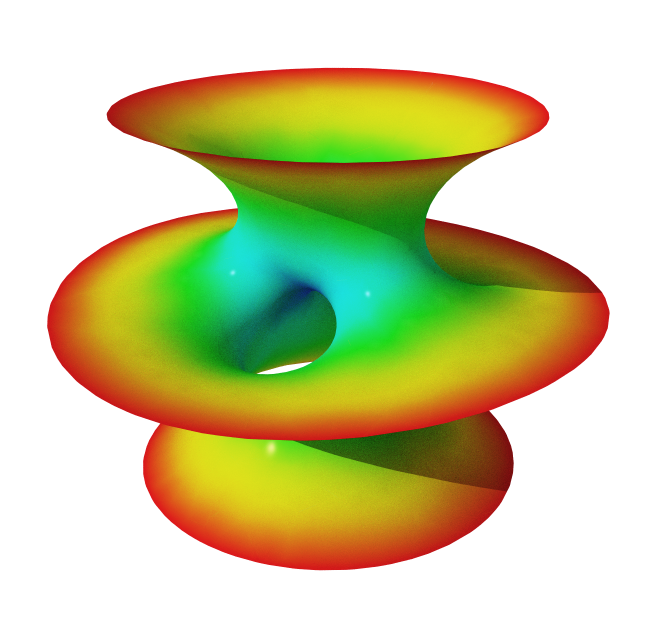
\includegraphics[width=0.35\textwidth]{exemplo-fig}
\caption*{Fonte: Wikipédia\footnotemark.}
\end{center}
\end{figure}
\footnotetext{\url{https://commons.wikimedia.org/wiki/File:Costa\%27s_Minimal_Surface.png}. Acesso em: 20 ago. 2021.}

A Superfície Costa\index{Superfície Costa} mostrada na Figura \ref{fig-exemplo} é uma superfície com curvatura média nula descoberta pelo matemático brasileiro Celso José da Costa.

\chapter{Considerações finais}

\citeonline{cordeiro} faz diversas considerações sobre a boa redação matemática. Recomendamos fortemente este texto.

\citeonline{anton} mostra uma referência com três autores. 

\citeonline{einstein} é um exemplo de referência com mais de três autores. 

%%%%%%%%%%%%%%%%%%%%%%%%%%%%%%%%%%%%%%%%%%%%%%%%%%%%%%%%%%%%%%%%%%%%%
% FIM DO EXEMPLO
%%%%%%%%%%%%%%%%%%%%%%%%%%%%%%%%%%%%%%%%%%%%%%%%%%%%%%%%%%%%%%%%%%%%%


%%%%%%%%%%%%%%%%%%%%%%%%%%%%%%%%%%%%%%%%%%%%%%%%%%%%%%%%%%%%%%%%%%%%%
% Elementos pós-textuais
% Inseridos após a parte textual, apresentam elementos que 
% complementam o trabalho.
%%%%%%%%%%%%%%%%%%%%%%%%%%%%%%%%%%%%%%%%%%%%%%%%%%%%%%%%%%%%%%%%%%%%%

% Referências
% Elemento OBRIGATÓRIO e deve ser elaborada de acordo com ABNT NBR 6023/2002.

% Utilize o BibTeX. As referências serão formatadas segundo a ABNT
% Colocar as referências no arquivo referencia.bib
% ATENÇÃO: NÃO UTILIZAR O COMANDO \nocite{*}
% TODAS AS REFERÊNCIAS DEVEM SER CITADAS NO TEXTO
% \cite[]{} ou \citeonline[]{}
\bibliography{referencias}
\addcontentsline{toc}{chapter}{REFER\^{E}NCIAS}

% Apêndice
% Elemento OPCIONAL que apresenta texto ou documento elaborado pelo autor, a fim de
% complementar sua argumentação. Deve ser precedido da palavra APÊNDICE,
% identificado por letras maiúsculas consecutivas, travessão e respectivo título.
% Comente o ambiente a seguir caso não fizer uso.

\begin{appendices}

\chapter{Parte que não será lida do trabalho}

Segue com o texto e partes que irão para o Apêndice. 

Remover caso não fizer uso.

\end{appendices}

% Anexo  --> a ser implementado sob demanda em razão do pouco uso
% Entrar em contato com seixas@ufscar.br
% Elemento OPCIONAL, apresenta um texto ou documento não elaborado pelo autor, que 
% serve de fundamentação, comprovação e ilustração. Deve ser precedido da palavra
% ANEXO, identificado por letras maiúsculas consecutivas, travessão e respectivo
% título.

% Índice
% Elemento OPCIONAL que apresenta lista de palavras ou frases, ordenadas segundo
% determinado critério, que localiza e remete para as informações contidas no texto.
% Deve ser elaborado de acordo com ABNT NBR 6034/2004.
% USO: ao longo do texto, após a palavra que irá para o Índice colocar 
% \index{<palavra>}
% Maiores detalhes em https://pt.overleaf.com/learn/latex/Indices
\printindex
 
% Licença Creative Commons - Repositório UFSCar
\cleardoublepage
\licenca

\end{document}
